\documentclass[a4paper,12pt, openany]{article}
\usepackage[a4paper, total={7in, 10in}]{geometry}
\usepackage{graphicx}
\usepackage{footnote}
\usepackage{subcaption}
\usepackage{pdfpages}
\usepackage{titling}
\graphicspath{ {./Figures/} }
\usepackage{multirow}
\usepackage{xcolor}
\usepackage{float}
\usepackage{polski}
\usepackage{hyperref}
\urlstyle{same}
\usepackage[polish]{babel}
\babelprovide[transforms = oneletter.nobreak]{polish}

\binoppenalty=10000
\relpenalty=10000
%opening

\pretitle{%
  \begin{center}
  \LARGE
  
\includegraphics[width=6cm]{logo}\\[\bigskipamount]
}
\posttitle{\end{center}}


%opening
\begin{document}

\title{\textbf{Automatyczny Ekspres do Herbaty} \\
    \begin{large}
     \textbf{Projekt Przejściowy}
    \end{large}
}

\author{\textbf{Łukasz Weber}}

\maketitle

\section{Wstęp}

Celem projektu jest zaprojektowanie automatycznego ekspresu do herbaty zawierającego minimum trzy osie ruchu. Aby osiągnąć ten cel konstrukcja musi spełniać następujące założenia:

\begin{itemize}
 \item Ekspres musi być w pełni automatyczny, gdzie jedynymi czynnościami wykonywanymi manualnie będzie okresowe dolanie wody do rezerwuaru, uzupełnienie suszu herbacianego w magazynku oraz usunięcie zgromadzonego zużytego suszu.
 \item Ekspres musi działać zarówno na susz herbaciany jak i torebki z herbatą
 \item Możliwość załadowania kilku rodzajów herbaty jednocześnie i wyboru, którą chcemy przygotować
 \item Kompaktowy rozmiar, aby można było go ustawić na kuchennym blacie
 \item Prosty i szybki montaż bez konieczności użycia specjalizowanych narzędzi, aby można było łatwo wyczyścić ekspres
\end{itemize}

Poniższy projekt skupia się tylko i wyłącznie na konstrukcji mechanicznej, elementy elektroniczne i układu sterowania nie są uwzględniane podczas projektowania.

\section{Rysunek Złożeniowy}

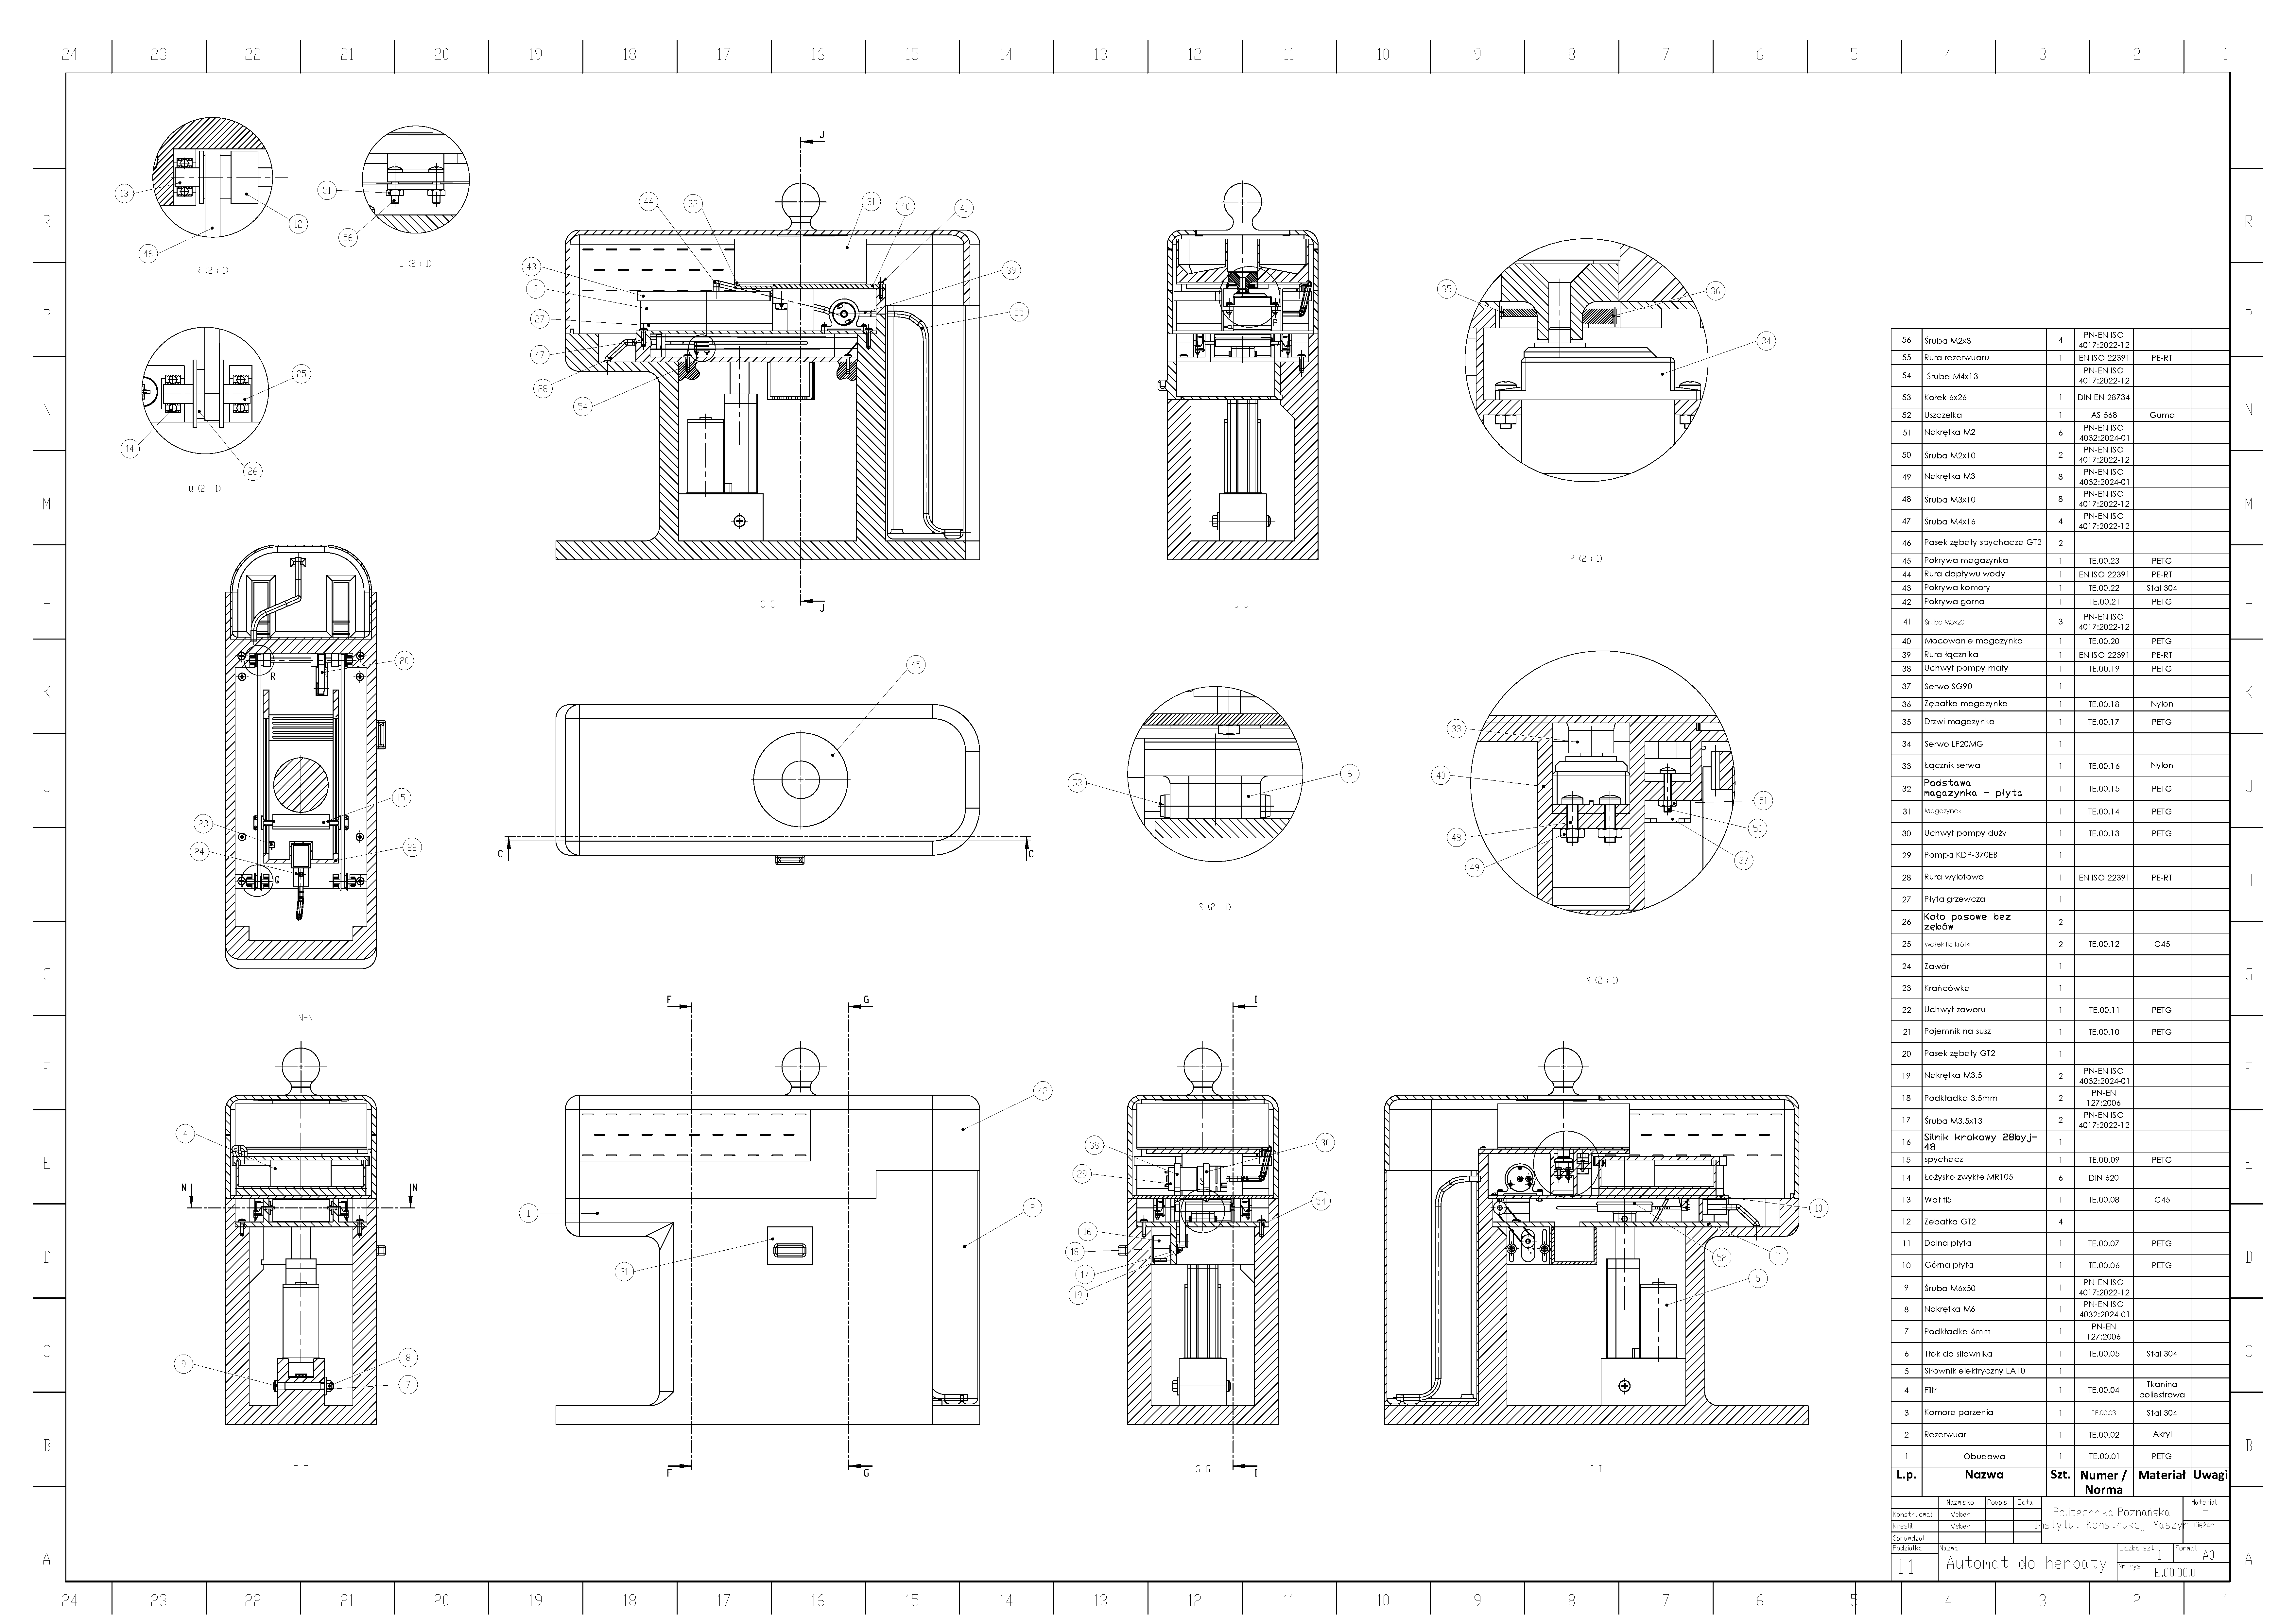
\includepdf[pages=1, fitpaper]{rysunek.pdf}

\section{Model 3D}
\begin{center}
 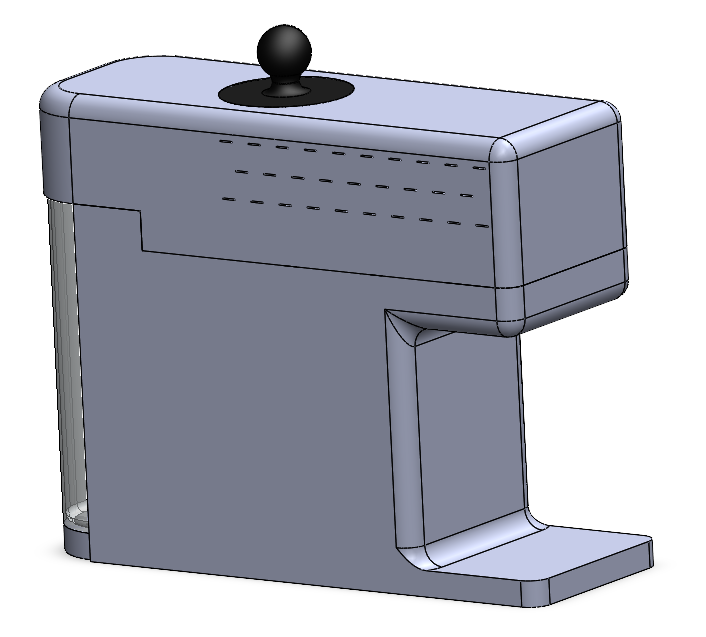
\includegraphics[width=0.7\textwidth]{model2.png}
 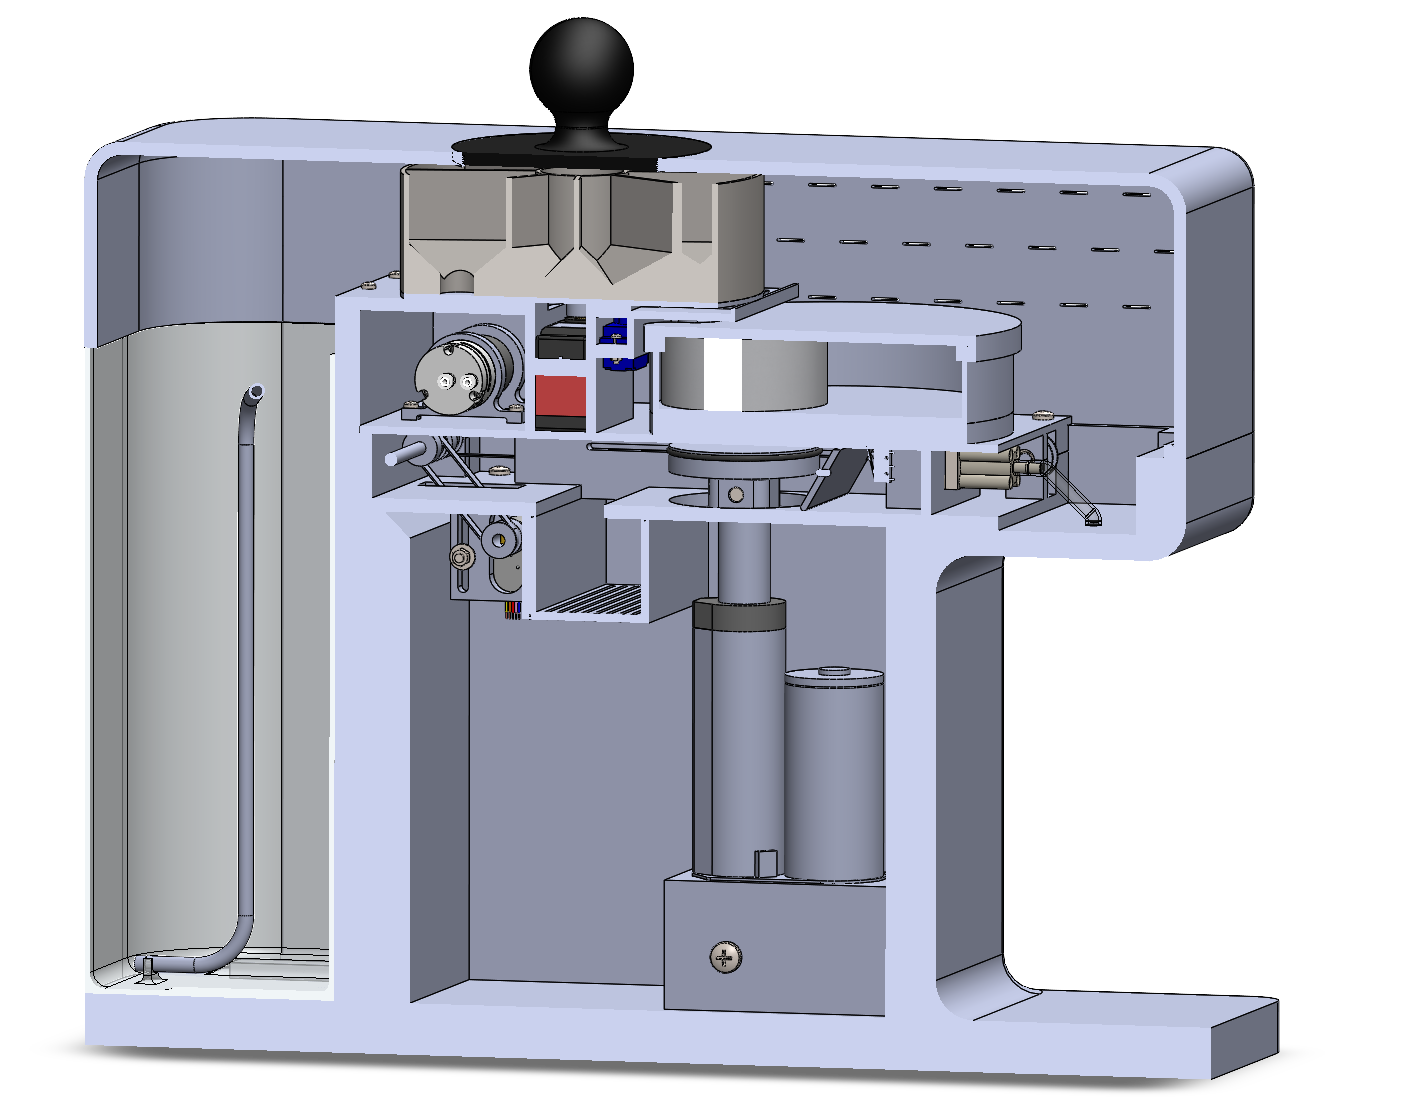
\includegraphics[width=0.9\textwidth]{model.png}
\end{center}




\section{Noty Katalogowe}
\subsection{Siłownik elektryczny LA10P}
\begin{center}
 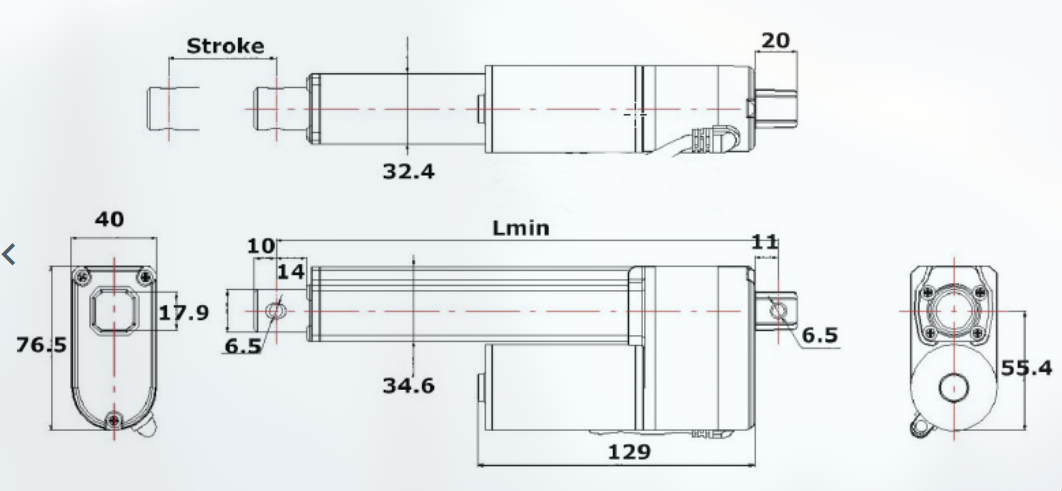
\includegraphics[width=\textwidth]{silownik.png}
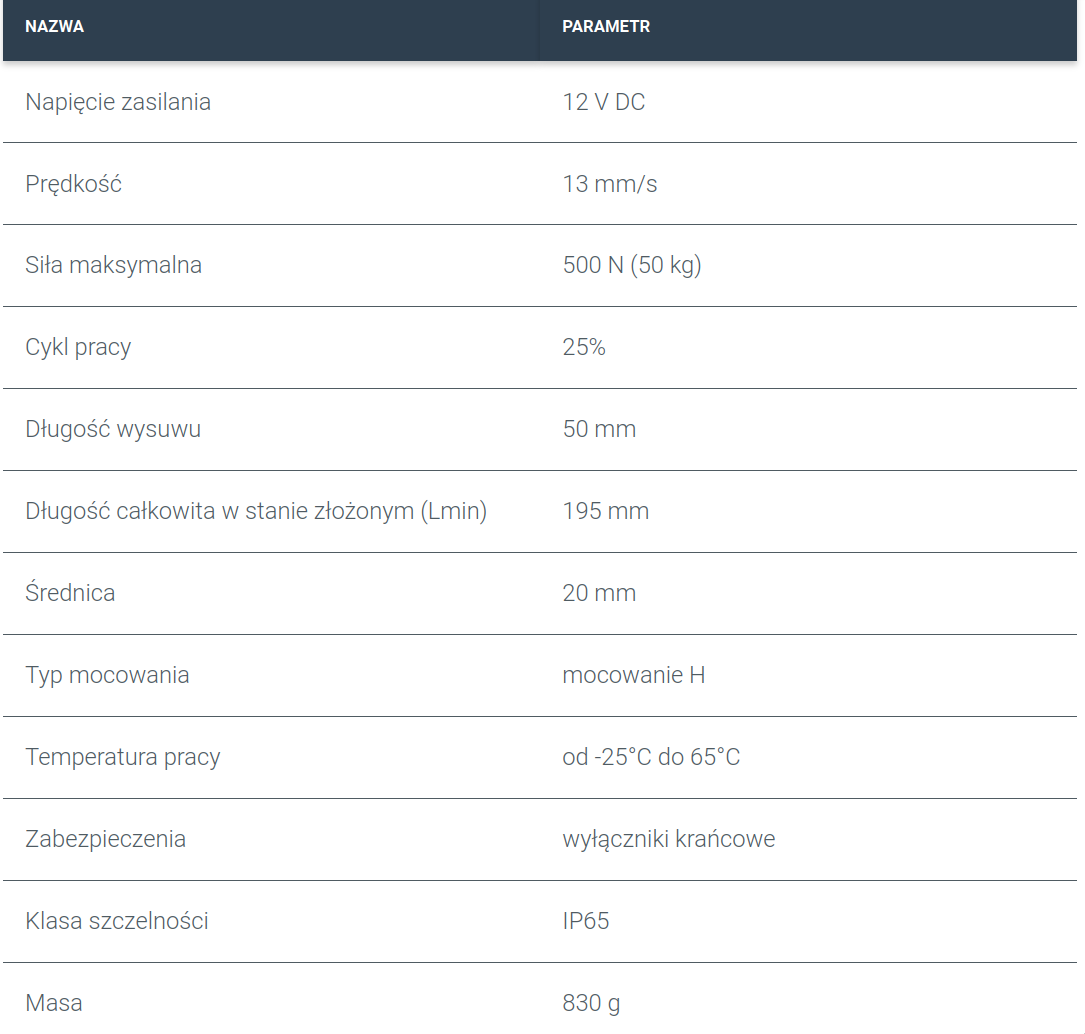
\includegraphics[width=0.9\textwidth]{silownik2.png}
\end{center}




\subsection{Koło zębate 20T GT2}
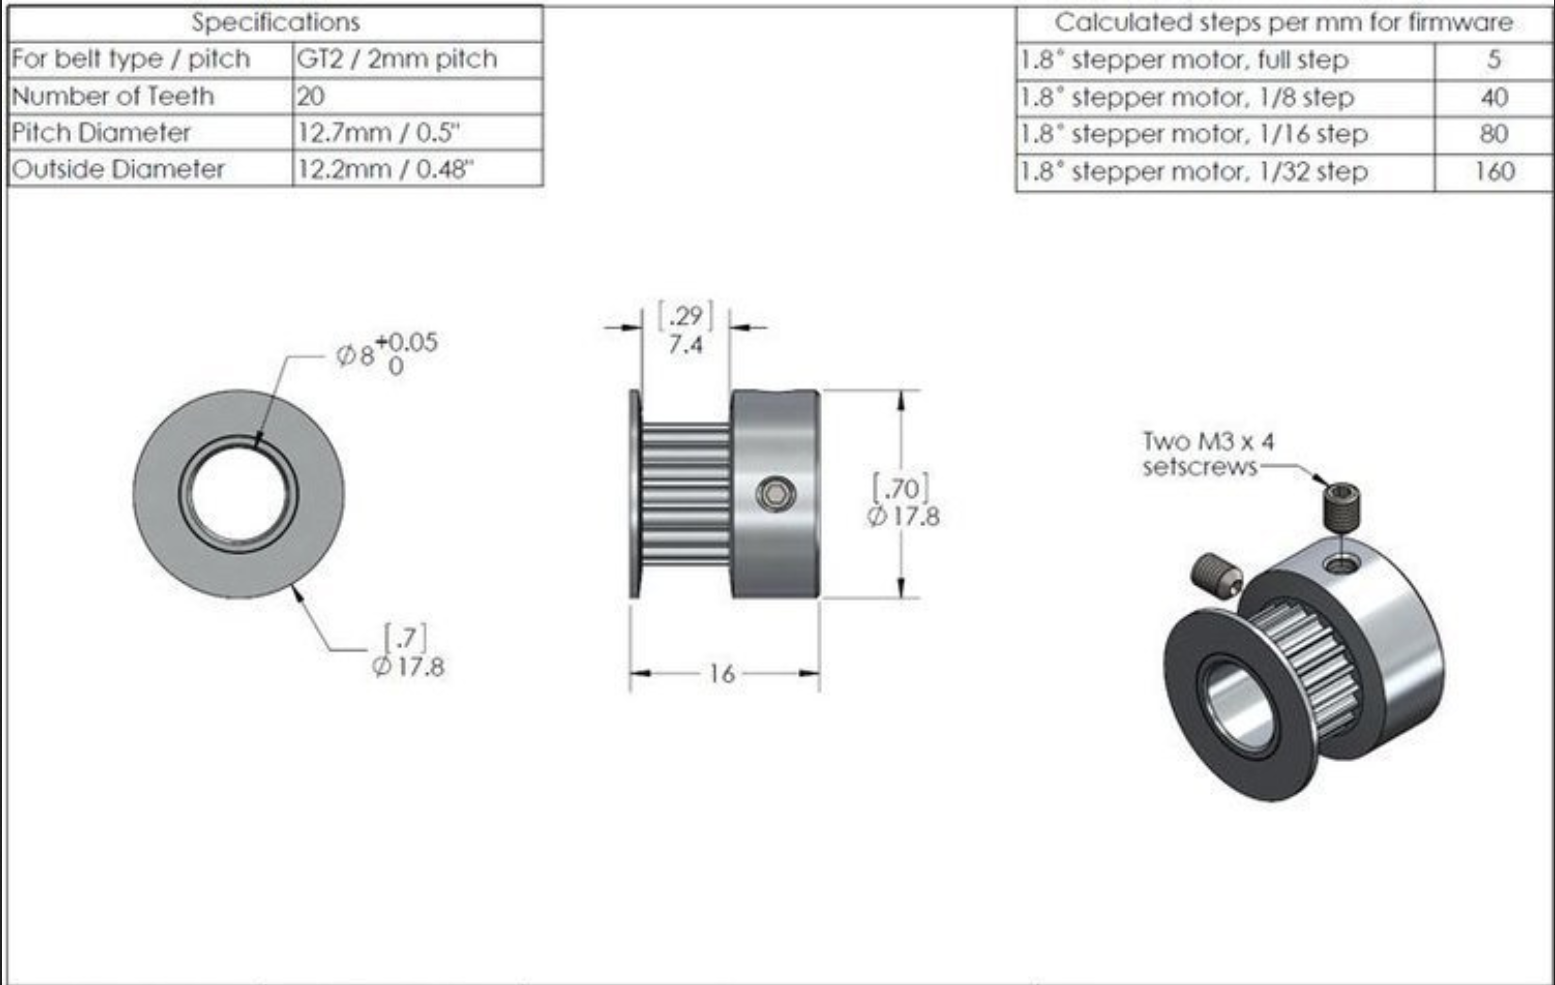
\includegraphics[width=\textwidth]{gt2.png}

\subsection{Łożysko MR105}
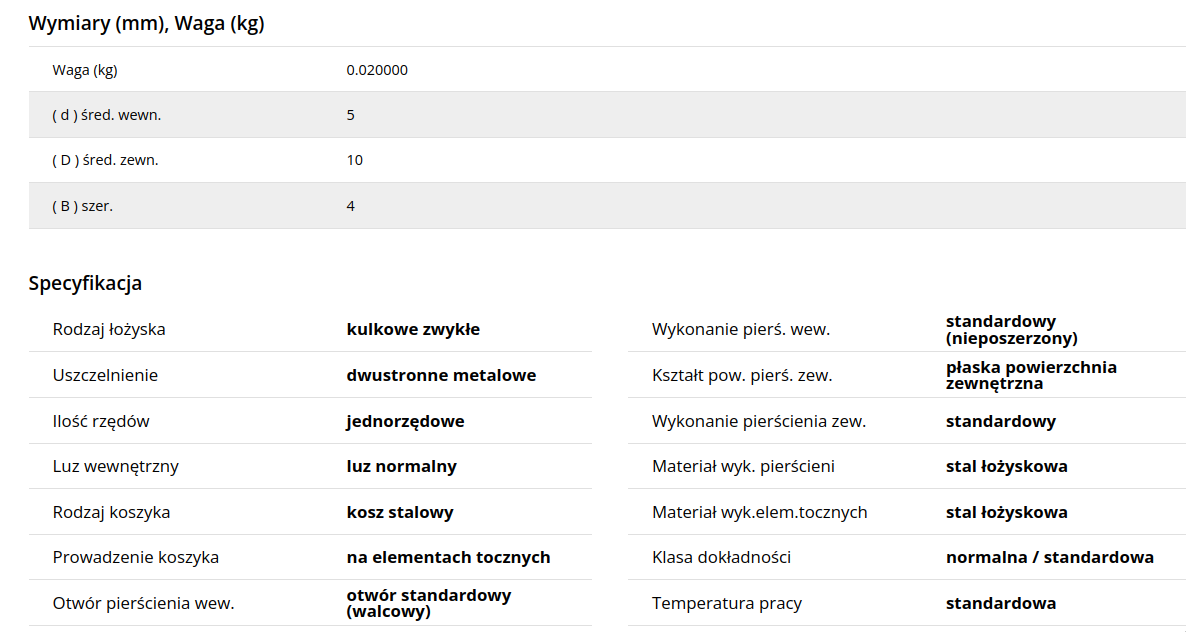
\includegraphics[width=\textwidth]{mr105.png}

\subsection{Silnik krokowy 28BYJ-48}
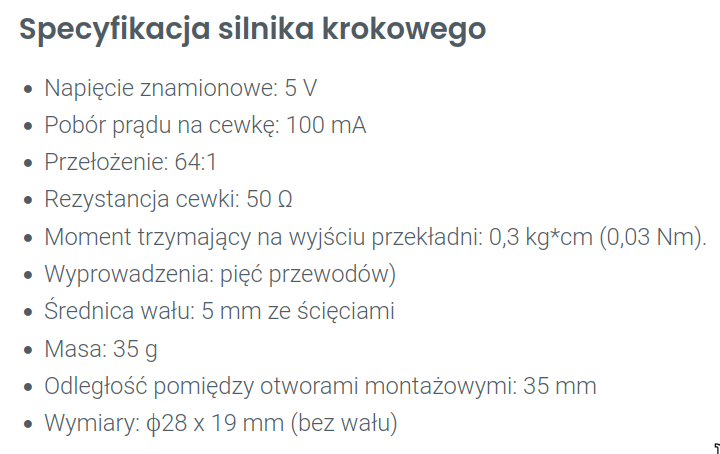
\includegraphics[width=\textwidth]{silnikkrokowy.png}

\subsection{Pompa KDP-370EB}
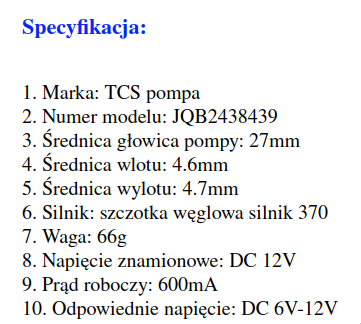
\includegraphics[width=0.6\textwidth]{pompa.png}

\subsection{Serwo LF20MG}
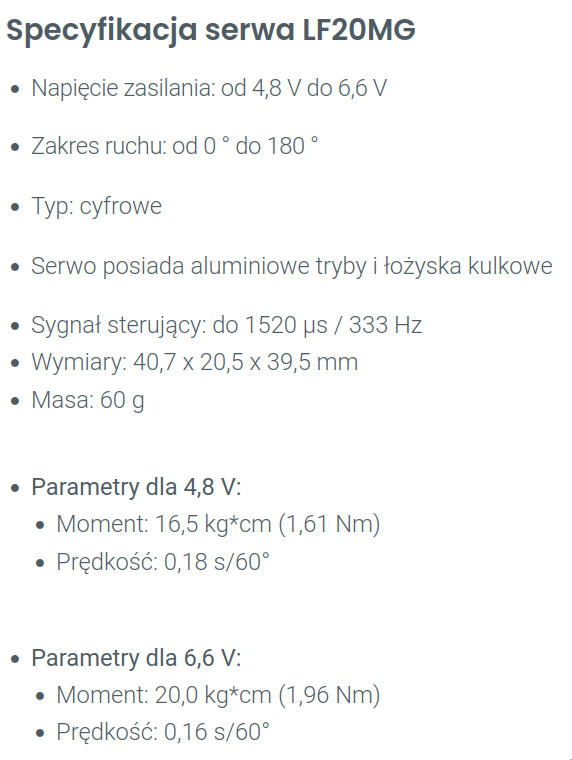
\includegraphics[width=0.6\textwidth]{serwolf.png}

\subsection{Serwo SG90}
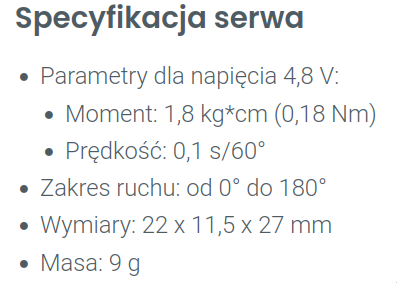
\includegraphics[width=0.6\textwidth]{serwosg.png}

\subsection{Pasek zębaty GT2}
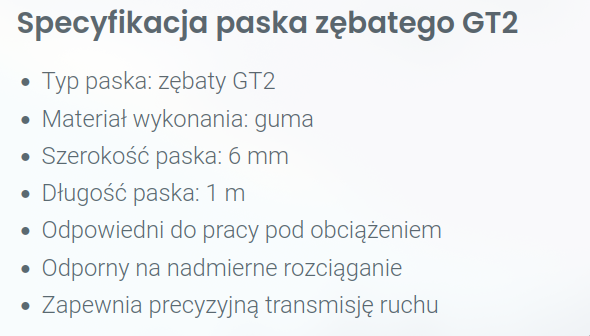
\includegraphics[width=\textwidth]{pasek.png}

\subsection{Krańcówka WK625}
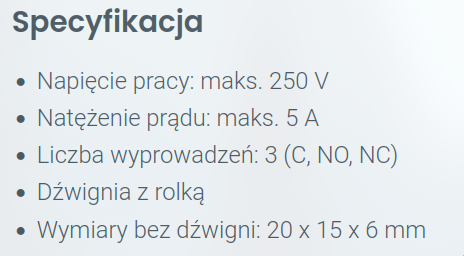
\includegraphics[width=\textwidth]{kran.png}

\subsection{Zawór S0626AV-D}
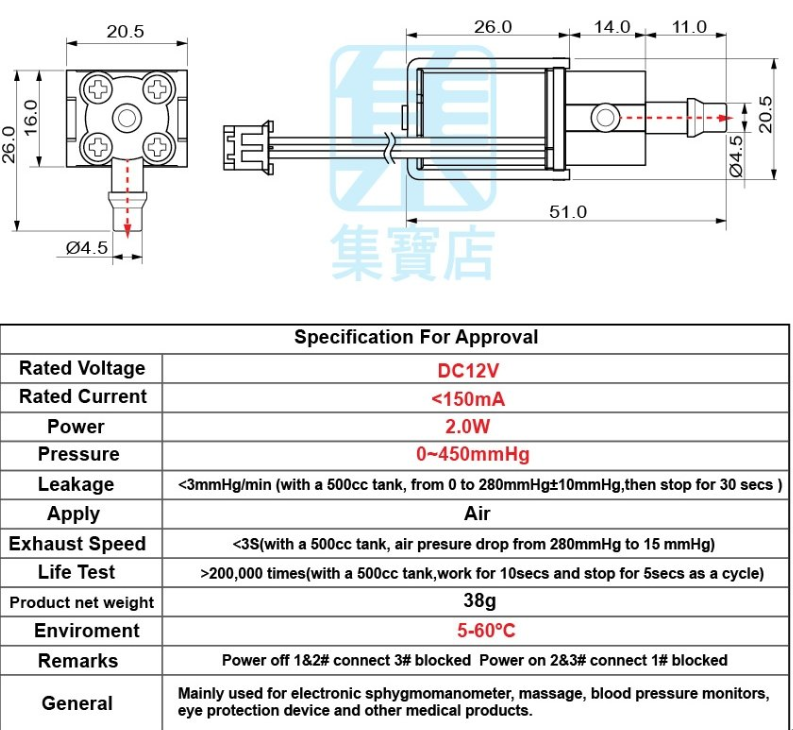
\includegraphics[width=0.8\textwidth]{zawor.png}

\subsection{Płyta grzewcza WEBO}
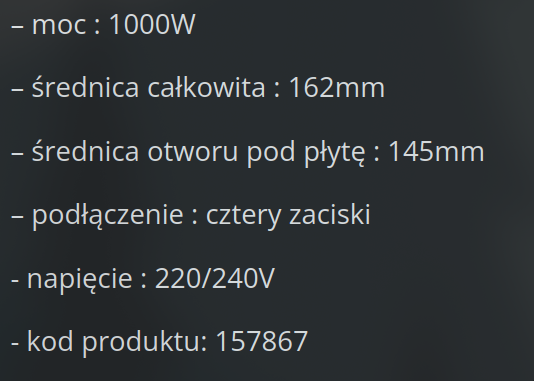
\includegraphics[width=0.7\textwidth]{plyta.png}


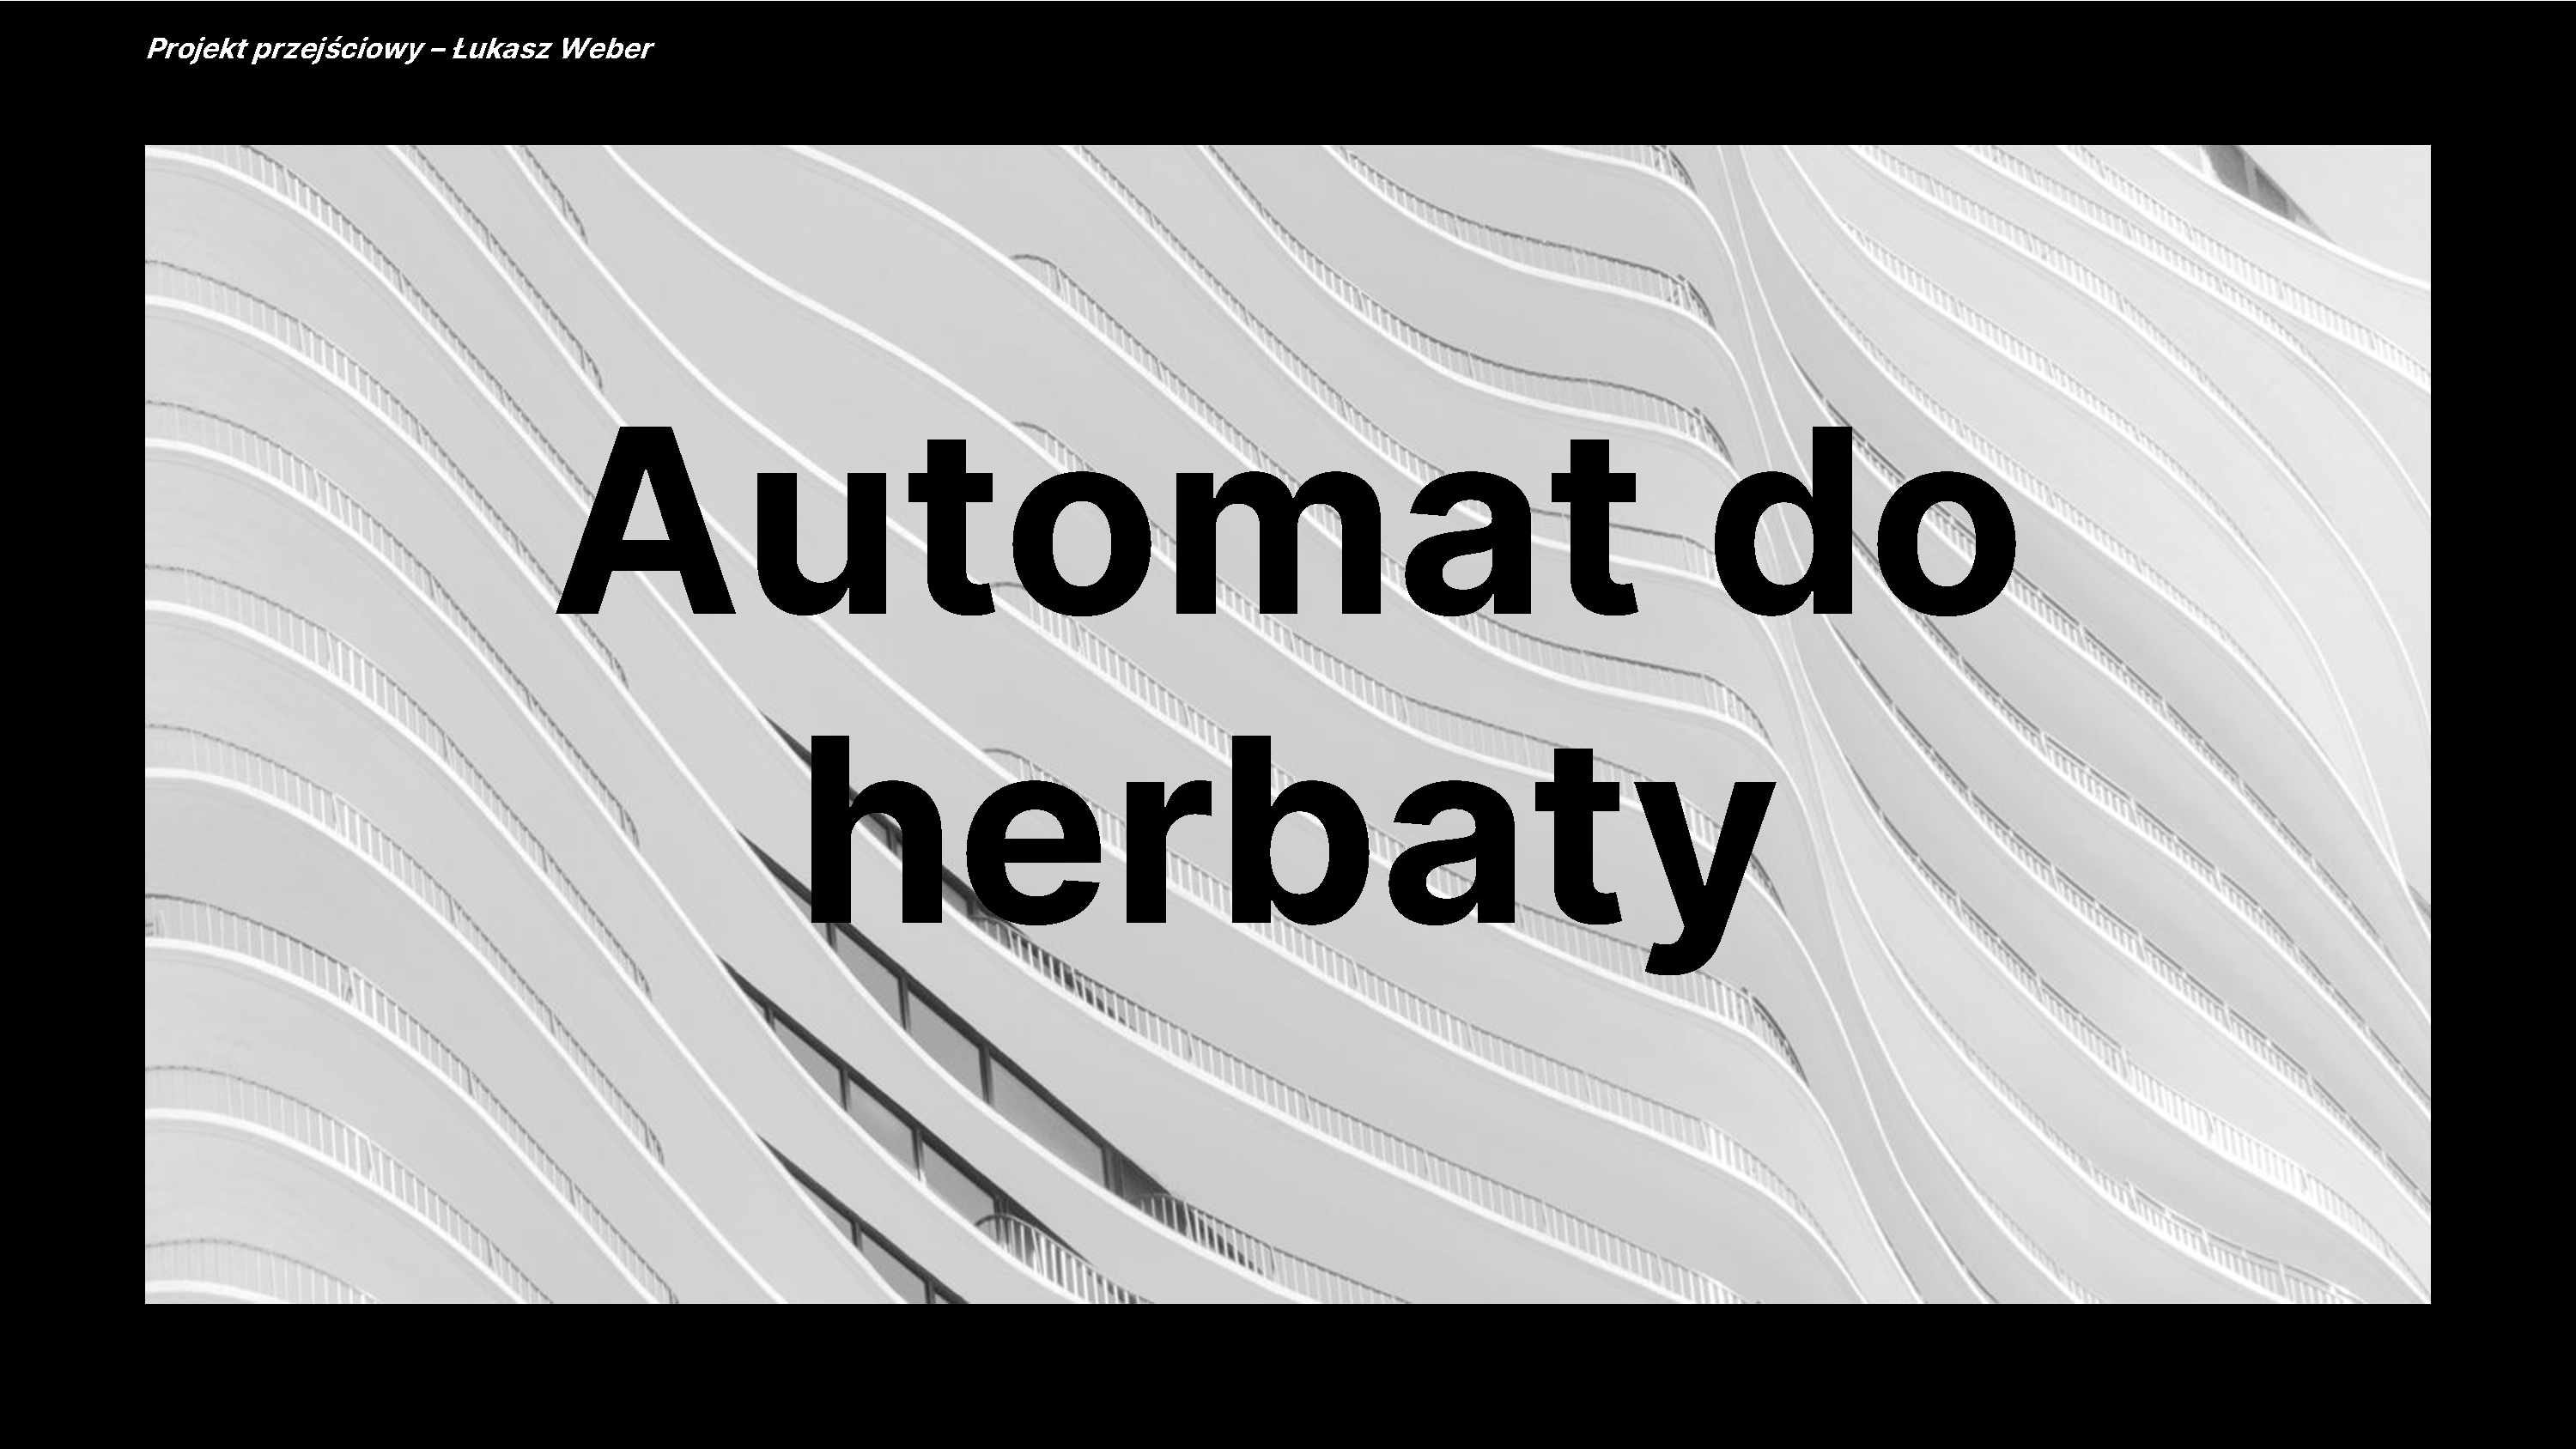
\includepdf[pages=-, fitpaper]{Prezentacja 1 revised.pdf}
\includepdf[pages=-, fitpaper]{Prezentacja 2.pdf}

\end{document}
